因此，对于固定的 $i_2$，条件分布 $\PP(X_1|X_2=i_2)\propto\begin{tikzpicture}[baseline=\baseline]
    \tikzset{tensor/.style = {minimum size = 0.5cm,shape = circle,thick,draw=black,inner sep = 0pt}, edge/.style = {thick,line width=.4mm},every loop/.style={}}
    \def\y{0.25}
    \def\x{0}
    \node[tensor,fill=blue!20!white] (T) at (\x,\y) {$\Tt$};
    \draw  node[fill = black,circle,inner sep=0pt,minimum size=4pt] (m_1) at (\x+0.5,\y-0.65) {};
    \draw[edge] (T) -- (\x-0.5,\y-0.65);
    \draw[edge](T) -- (\x,\y-0.75)node [very near end,below]
    {\scalebox{0.7}{\indcolor{$i_2$}}};
    \draw[edge](T) -- (m_1);
\end{tikzpicture}.$
\item 我们有 $\PP(i_3|i_1,i_2) = \frac{\PP(i_1,i_2,i_3)}{\PP(i_1,i_2)}=\frac{\PP(i_1,i_2,i_3)}{\sum_{i_3}\PP(i_1,i_2,i_3)}
=
\frac{\begin{tikzpicture}[baseline=\baseline]
    \tikzset{tensor/.style = {minimum size = 0.5cm,shape = circle,thick,draw=black,inner sep = 0pt}, edge/.style = {thick,line width=.4mm},every loop/.style={}}
    \def\x{0}
    \def\y{0}
    \node[tensor,fill=blue!20!white] (T) at (\x,\y) {$\Tt$};
    \draw[edge] (T) -- (\x-0.5,\y-0.65)node [very near end,below]
    {\scalebox{0.7}{\indcolor{$i_1$}}};
    \draw[edge](T) -- (\x,\y-0.75)node [very near end,below]
    {\scalebox{0.7}{\indcolor{$i_2$}}};
    \draw[edge](T) -- (\x+0.5,\y-0.65)node [very near end,below]
    {\scalebox{0.7}{\indcolor{$i_3$}}};
\end{tikzpicture}}{\begin{tikzpicture}[baseline=\baseline]
    \tikzset{tensor/.style = {minimum size = 0.5cm,shape = circle,thick,draw=black,inner sep = 0pt}, edge/.style = {thick,line width=.4mm},every loop/.style={}}
    \def\x{0}
    \def\y{0}
    \node[tensor,fill=blue!20!white] (T) at (\x,\y) {$\Tt$};
    \draw  node[fill = black,circle,inner sep=0pt,minimum size=4pt] (m_2) at (\x+0.5,\y-0.65) {};
    \draw[edge] (T) -- (\x-0.5,\y-0.65)node [very near end,below]
    {\scalebox{0.7}{\indcolor{$i_1$}}};
    \draw[edge](T) -- (m_2);
    \draw[edge](T) -- (\x,\y-0.75)node [very near end,below]
    {\scalebox{0.7}{\indcolor{$i_2$}}};
\end{tikzpicture}},
$
对任意 $i_1, i_2$ 和 $i_3$ 成立。

因此，对于固定的 $i_1$ 和 $ i_2$，条件分布 $\PP(X_3|X_1=i_1, X_2 = i_2)\propto\begin{tikzpicture}[baseline=\baseline]
    \tikzset{tensor/.style = {minimum size = 0.5cm,shape = circle,thick,draw=black,inner sep = 0pt}, edge/.style = {thick,line width=.4mm},every loop/.style={}}
    \def\y{0.25}
    \def\x{0}
    \node[tensor,fill=blue!20!white] (T) at (\x,\y) {$\Tt$};
    \draw[edge] (T) -- (\x-0.5,\y-0.65)node [very near end,below]
    {\scalebox{0.7}{\indcolor{$i_1$}}};
    \draw[edge](T) -- (\x,\y-0.75)node [very near end,below]
    {\scalebox{0.7}{\indcolor{$i_2$}}};
    \draw[edge](T) -- (\x+0.5,\y-0.65);
\end{tikzpicture}.$ 
\end{enumerate}
\subsubsection{概率分布的张量列参数化}
如第~\ref{chapter:tensor-decomposition} 章所见，处理高阶张量的计算代价很高，因为元素个数随张量的阶指数增长。表示联合概率分布的张量也是如此：张量表示的规模随随机变量的个数指数增长。解决这一问题的一个途径，是把概率张量参数化为低秩张量网络。

这里我们说明如何用张量列分解做到这一点。其他分解模型同样可行，但张量列格式尤为有趣，并已在量子物理中非常成功地用于建模多体系统~\citep{TensorNetworkOrg}。

设 $\Tt\in\RR^{d_1\times\cdots\times d_N}$ 为以张量列格式参数化的概率张量： 
\begin{center}
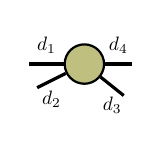
\begin{tikzpicture}[baseline=-0.5ex]
    \tikzset{tensor/.style = {minimum size = 0.5cm,shape = circle,thick,draw=black,inner sep = 0pt}, edge/.style = {thick,line width=.4mm},every loop/.style={}}
    \def\x{6}
    \def\y{0}
     \node[tensor,fill=green!50!red!50!white] (B) at (\x+1,\y) {$\Tt$};
    \draw[edge] (B) -- (\x+0.3,0) node [midway,above] {\scalebox{0.7}{\dimcolor{$d_1$}}};
    \draw[edge] (B) -- (\x+1.6,0) node [midway,above] {\scalebox{0.7}{\dimcolor{$d_4$}}};
    \draw[edge] (B) -- (\x+0.4,-0.3) node [midway, below] {\scalebox{0.7}{\dimcolor{$d_2$}}};
    \draw[edge] (B) -- (\x+1.5,-0.4)node [midway, below] {\scalebox{0.7}{\dimcolor{$d_3$}}};
\end{tikzpicture}
=
\begin{tikzpicture}[baseline=\baseline]
    \tikzset{tensor/.style = {minimum size = 0.5cm,shape = circle,thick,draw=black,inner sep = 0pt}, edge/.style   = {thick,line width=.4mm},every loop/.style={}}
    \def\y{0}
    \def\x{0}
  \node[tensor,fill=red!30!white] (D) at (\x-1,\y){$\Gt_1$};
  \node[tensor,fill=red!50!white] (A) at (\x,\y){\scalebox{0.85}{$\Gt_2$}};
  \node[tensor,fill=blue!50!white] (B) at (\x+1,\y){$\Gt_3$};
   \node[tensor,fill=blue!20!white] (C) at (\x+2,\y){$\Gt_4$};
    \draw[edge](A) -- (\x,\y-0.7)node [midway,left] {\edgelabel{$d_2$}};
    \draw[edge](B) -- (\x+1,\y-0.7)node [midway,left] {\edgelabel{$d_3$}};
    \draw[edge](C) -- (\x+2,\y-0.7)node [midway,left] {\edgelabel{$d_4$}};
     \draw[edge](D) -- (\x-1,\y-0.7)node [midway,left] {\edgelabel{$d_1$}};
    \draw[edge](D) -- (A) node [midway,above] {\edgelabel{$R_1$}};
    \draw[edge](A) -- (B) node [midway,above] {\edgelabel{$R_2$}};
    \draw[edge](B) -- (C) node [midway,above] {\edgelabel{$R_3$}};
\end{tikzpicture}.
\end{center}

由于 $\Tt$ 表示一个概率分布，它的元素必须非负，且总和为一。
在机器学习场景中，我们要针对某个损失函数~（如对数似然）来优化核心张量，此时可以对核心张量 $\Gt_1,\cdots,\Gt_N$ 施加若干约束以保证这两条性质。 
要保证 $\Tt$ 的元素非负，一个简单的办法是约束核心张量的元素非负，或者对所有核心张量的元素逐分量地施加一个取值非负的“激活”函数。另一种做法源于量子物理：假设 $\Tt$ 的元素是概率的平方根，而非概率本身： $\Tt_{i_1,\cdots,i_N} = \sqrt{\PP(X_1=i_1,\cdots,X_N=i_N)}$。当 $\Tt$ 处于 TT 格式时，这对应于如下张量网络：
$$
\PP(X_1=i_1,\cdots,X_4=i_4) = (\Tt_{i_1,\cdots,i_4})^2 = 
\begin{tikzpicture}[baseline=\baseline]
    \tikzset{tensor/.style = {minimum size = 0.5cm,shape = circle,thick,draw=black,inner sep = 0pt}, edge/.style   = {thick,line width=.4mm},every loop/.style={}}
    \def\y{-0.35}
    \def\x{0}
  \node[tensor,fill=red!30!white] (D) at (\x-1,\y){$\Gt_1$};
  \node[tensor,fill=red!50!white] (A) at (\x,\y){\scalebox{0.85}{$\Gt_2$}};
  \node[tensor,fill=blue!50!white] (B) at (\x+1,\y){$\Gt_3$};
   \node[tensor,fill=blue!20!white] (C) at (\x+2,\y){$\Gt_4$};
   \node[tensor,fill=red!30!white] (G1) at (\x-1,\y+0.85){$\Gt_1$};
  \node[tensor,fill=red!50!white] (G2) at (\x,\y+0.85){\scalebox{0.85}{$\Gt_2$}};
  \node[tensor,fill=blue!50!white] (G3) at (\x+1,\y+0.85){$\Gt_3$};
   \node[tensor,fill=blue!20!white] (G4) at (\x+2,\y+0.85){$\Gt_4$};
    \draw[edge](G1) -- (\x-1,\y+1.65)node [very near end, above]{\scalebox{0.7} {\indcolor{$i_1$}}};
    \draw[edge](G2) -- (\x,\y+1.65)node [very near end, above]{\scalebox{0.7} {\indcolor{$i_2$}}};
    \draw[edge](G3) -- (\x+1,\y+1.65)node [very near end, above]{\scalebox{0.7}{\indcolor{$i_3$}}};
    \draw[edge](G4) -- (\x+2,\y+1.65)node [very near end, above]{\scalebox{0.7}{\indcolor{$i_4$}}};
    \draw[edge](G1) -- (G2)node [midway,above] {\edgelabel{$R_1$}};
    \draw[edge](G2) -- (G3)node [midway,above] {\edgelabel{$R_2$}};
    \draw[edge](G3) -- (G4)node [midway,above] {\edgelabel{$R_3$}};
    \draw[edge](A) -- (\x,\y-0.7)node [very near end, below] {\scalebox{0.7}{\indcolor{$i_2$}}};
    \draw[edge](B) -- (\x+1,\y-0.7)node [very near end, below]{\scalebox{0.7} {\indcolor{$i_3$}}};
    \draw[edge](C) -- (\x+2,\y-0.7)node [very near end, below] {\scalebox{0.7}{\indcolor{$i_4$}}};
     \draw[edge](D) -- (\x-1,\y-0.7)node [very near end, below] {\scalebox{0.7}{\indcolor{$i_1$}}};
    \draw[edge](D) -- (A) node [midway,above] {\edgelabel{$R_1$}};
    \draw[edge](A) -- (B) node [midway,above] {\edgelabel{$R_2$}};
    \draw[edge](B) -- (C) node [midway,above] {\edgelabel{$R_3$}};
\end{tikzpicture}
.
$$

